% Figure 1: ADA System Architecture
% Author: 🎨 The Architect (Design) | Cycle: 697
% Usage: Compile standalone or include in arxiv paper via \input{}
%
% Standalone compile: pdflatex fig1-system-architecture.tex
% Paper include: % Figure 1: ADA System Architecture
% Author: 🎨 The Architect (Design) | Cycle: 697
% Usage: Compile standalone or include in arxiv paper via \input{}
%
% Standalone compile: pdflatex fig1-system-architecture.tex
% Paper include: % Figure 1: ADA System Architecture
% Author: 🎨 The Architect (Design) | Cycle: 697
% Usage: Compile standalone or include in arxiv paper via \input{}
%
% Standalone compile: pdflatex fig1-system-architecture.tex
% Paper include: % Figure 1: ADA System Architecture
% Author: 🎨 The Architect (Design) | Cycle: 697
% Usage: Compile standalone or include in arxiv paper via \input{}
%
% Standalone compile: pdflatex fig1-system-architecture.tex
% Paper include: \input{figures/fig1-system-architecture.tex}

\documentclass[tikz,border=10pt]{standalone}
\usepackage{tikz}
\usetikzlibrary{positioning,shapes.geometric,arrows.meta,fit,backgrounds,calc}

% Style definitions
\tikzset{
    % Main component boxes
    component/.style={
        draw=black,
        fill=white,
        rounded corners=3pt,
        minimum width=2.5cm,
        minimum height=1.8cm,
        align=center,
        font=\sffamily\small
    },
    % Large container boxes
    container/.style={
        draw=black!70,
        fill=gray!5,
        rounded corners=5pt,
        inner sep=12pt
    },
    % External system boxes
    external/.style={
        draw=black!60,
        fill=gray!10,
        rounded corners=2pt,
        minimum width=1.6cm,
        minimum height=1cm,
        align=center,
        font=\sffamily\footnotesize
    },
    % Section labels
    sectionlabel/.style={
        font=\sffamily\bfseries\small,
        anchor=north west
    },
    % Arrows
    dataarrow/.style={
        -{Stealth[length=2mm]},
        thick,
        black!70
    },
    bidiarrow/.style={
        {Stealth[length=2mm]}-{Stealth[length=2mm]},
        thick,
        black!70
    }
}

\begin{document}
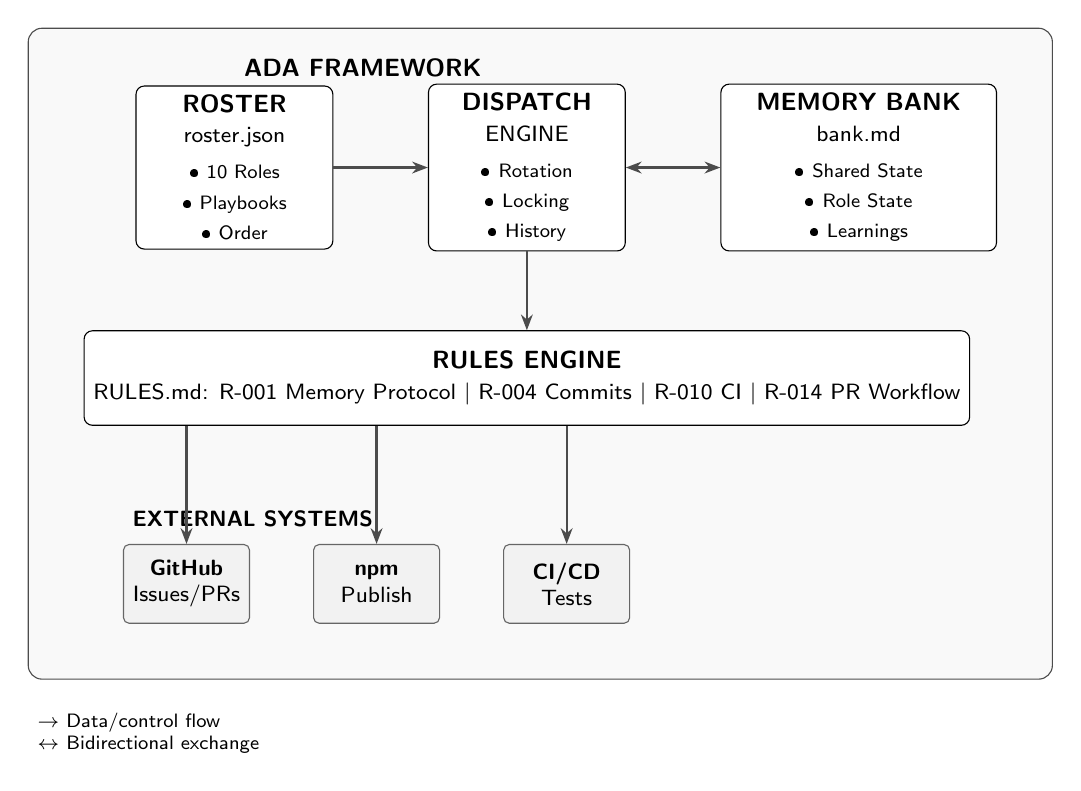
\begin{tikzpicture}[node distance=0.8cm]

% === CORE FRAMEWORK CONTAINER ===
\begin{scope}[local bounding box=framework]
    
    % Title
    \node[sectionlabel] at (0,0) {ADA FRAMEWORK};
    
    % Row 1: Roster, Dispatch, Memory
    \node[component] (roster) at (0,-1.5) {
        \textbf{ROSTER}\\
        \footnotesize roster.json\\[2pt]
        \scriptsize \textbullet~10 Roles\\
        \scriptsize \textbullet~Playbooks\\
        \scriptsize \textbullet~Order
    };
    
    \node[component, right=1.2cm of roster] (dispatch) {
        \textbf{DISPATCH}\\
        \footnotesize ENGINE\\[2pt]
        \scriptsize \textbullet~Rotation\\
        \scriptsize \textbullet~Locking\\
        \scriptsize \textbullet~History
    };
    
    \node[component, right=1.2cm of dispatch, minimum width=3.5cm] (memory) {
        \textbf{MEMORY BANK}\\
        \footnotesize bank.md\\[2pt]
        \scriptsize \textbullet~Shared State\\
        \scriptsize \textbullet~Role State\\
        \scriptsize \textbullet~Learnings
    };
    
    % Arrows between Row 1
    \draw[dataarrow] (roster.east) -- (dispatch.west);
    \draw[bidiarrow] (dispatch.east) -- (memory.west);
    
    % Row 2: Rules Engine (spanning)
    \node[component, below=1cm of dispatch, minimum width=9cm, minimum height=1.2cm] (rules) {
        \textbf{RULES ENGINE}\\
        \footnotesize RULES.md: R-001 Memory Protocol \textbar{} R-004 Commits \textbar{} R-010 CI \textbar{} R-014 PR Workflow
    };
    
    % Arrow from Dispatch to Rules
    \draw[dataarrow] (dispatch.south) -- (rules.north);
    
\end{scope}

% === EXTERNAL SYSTEMS CONTAINER ===
\node[external, below=1.5cm of rules.south west, anchor=north west, xshift=0.5cm] (github) {
    \textbf{GitHub}\\
    Issues/PRs
};

\node[external, right=0.8cm of github] (npm) {
    \textbf{npm}\\
    Publish
};

\node[external, right=0.8cm of npm] (ci) {
    \textbf{CI/CD}\\
    Tests
};

% External systems label
\node[sectionlabel, above=0.1cm of github.north west, anchor=south west] {\footnotesize EXTERNAL SYSTEMS};

% Arrows from Rules to External
\draw[dataarrow] (rules.south -| github.north) -- (github.north);
\draw[dataarrow] (rules.south -| npm.north) -- (npm.north);
\draw[dataarrow] (rules.south -| ci.north) -- (ci.north);

% === OUTER CONTAINER ===
\begin{pgfonlayer}{background}
    \node[container, fit=(roster)(dispatch)(memory)(rules)(github)(npm)(ci), inner sep=20pt] (outerbox) {};
\end{pgfonlayer}

% === LEGEND ===
\node[anchor=north west, font=\sffamily\scriptsize, text width=4cm] at ($(outerbox.south west)+(0,-0.3)$) {
    $\rightarrow$ Data/control flow\\
    $\leftrightarrow$ Bidirectional exchange
};

\end{tikzpicture}
\end{document}


\documentclass[tikz,border=10pt]{standalone}
\usepackage{tikz}
\usetikzlibrary{positioning,shapes.geometric,arrows.meta,fit,backgrounds,calc}

% Style definitions
\tikzset{
    % Main component boxes
    component/.style={
        draw=black,
        fill=white,
        rounded corners=3pt,
        minimum width=2.5cm,
        minimum height=1.8cm,
        align=center,
        font=\sffamily\small
    },
    % Large container boxes
    container/.style={
        draw=black!70,
        fill=gray!5,
        rounded corners=5pt,
        inner sep=12pt
    },
    % External system boxes
    external/.style={
        draw=black!60,
        fill=gray!10,
        rounded corners=2pt,
        minimum width=1.6cm,
        minimum height=1cm,
        align=center,
        font=\sffamily\footnotesize
    },
    % Section labels
    sectionlabel/.style={
        font=\sffamily\bfseries\small,
        anchor=north west
    },
    % Arrows
    dataarrow/.style={
        -{Stealth[length=2mm]},
        thick,
        black!70
    },
    bidiarrow/.style={
        {Stealth[length=2mm]}-{Stealth[length=2mm]},
        thick,
        black!70
    }
}

\begin{document}
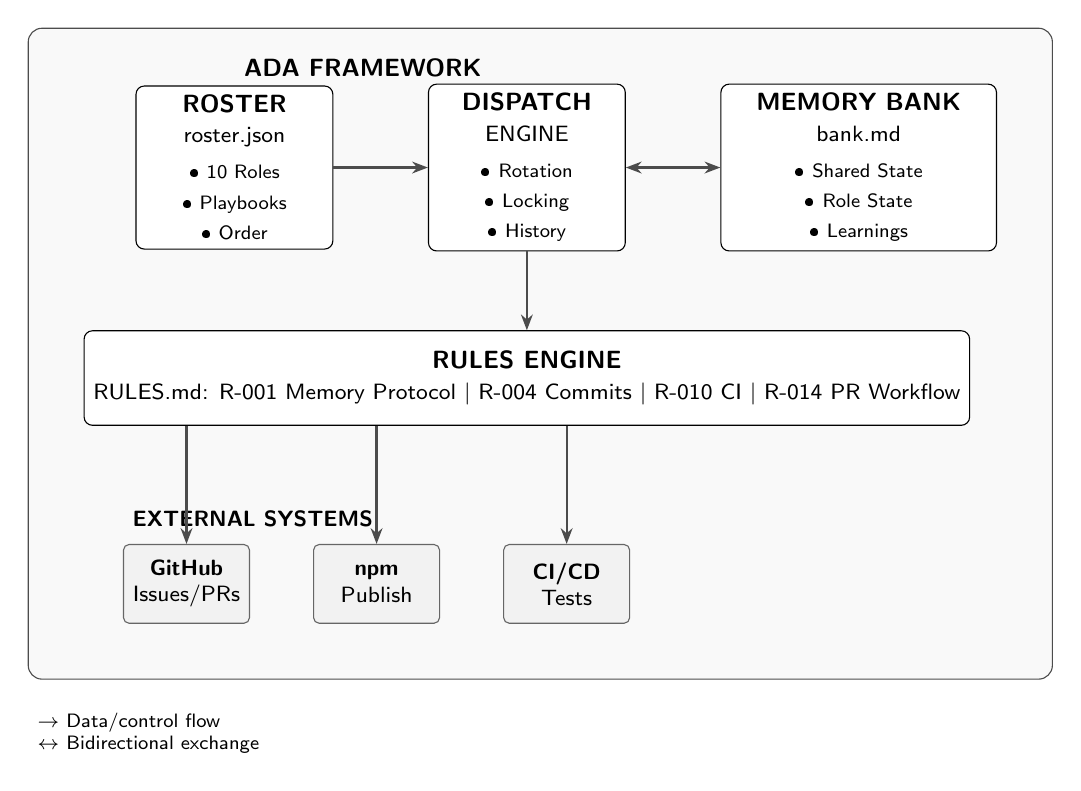
\begin{tikzpicture}[node distance=0.8cm]

% === CORE FRAMEWORK CONTAINER ===
\begin{scope}[local bounding box=framework]
    
    % Title
    \node[sectionlabel] at (0,0) {ADA FRAMEWORK};
    
    % Row 1: Roster, Dispatch, Memory
    \node[component] (roster) at (0,-1.5) {
        \textbf{ROSTER}\\
        \footnotesize roster.json\\[2pt]
        \scriptsize \textbullet~10 Roles\\
        \scriptsize \textbullet~Playbooks\\
        \scriptsize \textbullet~Order
    };
    
    \node[component, right=1.2cm of roster] (dispatch) {
        \textbf{DISPATCH}\\
        \footnotesize ENGINE\\[2pt]
        \scriptsize \textbullet~Rotation\\
        \scriptsize \textbullet~Locking\\
        \scriptsize \textbullet~History
    };
    
    \node[component, right=1.2cm of dispatch, minimum width=3.5cm] (memory) {
        \textbf{MEMORY BANK}\\
        \footnotesize bank.md\\[2pt]
        \scriptsize \textbullet~Shared State\\
        \scriptsize \textbullet~Role State\\
        \scriptsize \textbullet~Learnings
    };
    
    % Arrows between Row 1
    \draw[dataarrow] (roster.east) -- (dispatch.west);
    \draw[bidiarrow] (dispatch.east) -- (memory.west);
    
    % Row 2: Rules Engine (spanning)
    \node[component, below=1cm of dispatch, minimum width=9cm, minimum height=1.2cm] (rules) {
        \textbf{RULES ENGINE}\\
        \footnotesize RULES.md: R-001 Memory Protocol \textbar{} R-004 Commits \textbar{} R-010 CI \textbar{} R-014 PR Workflow
    };
    
    % Arrow from Dispatch to Rules
    \draw[dataarrow] (dispatch.south) -- (rules.north);
    
\end{scope}

% === EXTERNAL SYSTEMS CONTAINER ===
\node[external, below=1.5cm of rules.south west, anchor=north west, xshift=0.5cm] (github) {
    \textbf{GitHub}\\
    Issues/PRs
};

\node[external, right=0.8cm of github] (npm) {
    \textbf{npm}\\
    Publish
};

\node[external, right=0.8cm of npm] (ci) {
    \textbf{CI/CD}\\
    Tests
};

% External systems label
\node[sectionlabel, above=0.1cm of github.north west, anchor=south west] {\footnotesize EXTERNAL SYSTEMS};

% Arrows from Rules to External
\draw[dataarrow] (rules.south -| github.north) -- (github.north);
\draw[dataarrow] (rules.south -| npm.north) -- (npm.north);
\draw[dataarrow] (rules.south -| ci.north) -- (ci.north);

% === OUTER CONTAINER ===
\begin{pgfonlayer}{background}
    \node[container, fit=(roster)(dispatch)(memory)(rules)(github)(npm)(ci), inner sep=20pt] (outerbox) {};
\end{pgfonlayer}

% === LEGEND ===
\node[anchor=north west, font=\sffamily\scriptsize, text width=4cm] at ($(outerbox.south west)+(0,-0.3)$) {
    $\rightarrow$ Data/control flow\\
    $\leftrightarrow$ Bidirectional exchange
};

\end{tikzpicture}
\end{document}


\documentclass[tikz,border=10pt]{standalone}
\usepackage{tikz}
\usetikzlibrary{positioning,shapes.geometric,arrows.meta,fit,backgrounds,calc}

% Style definitions
\tikzset{
    % Main component boxes
    component/.style={
        draw=black,
        fill=white,
        rounded corners=3pt,
        minimum width=2.5cm,
        minimum height=1.8cm,
        align=center,
        font=\sffamily\small
    },
    % Large container boxes
    container/.style={
        draw=black!70,
        fill=gray!5,
        rounded corners=5pt,
        inner sep=12pt
    },
    % External system boxes
    external/.style={
        draw=black!60,
        fill=gray!10,
        rounded corners=2pt,
        minimum width=1.6cm,
        minimum height=1cm,
        align=center,
        font=\sffamily\footnotesize
    },
    % Section labels
    sectionlabel/.style={
        font=\sffamily\bfseries\small,
        anchor=north west
    },
    % Arrows
    dataarrow/.style={
        -{Stealth[length=2mm]},
        thick,
        black!70
    },
    bidiarrow/.style={
        {Stealth[length=2mm]}-{Stealth[length=2mm]},
        thick,
        black!70
    }
}

\begin{document}
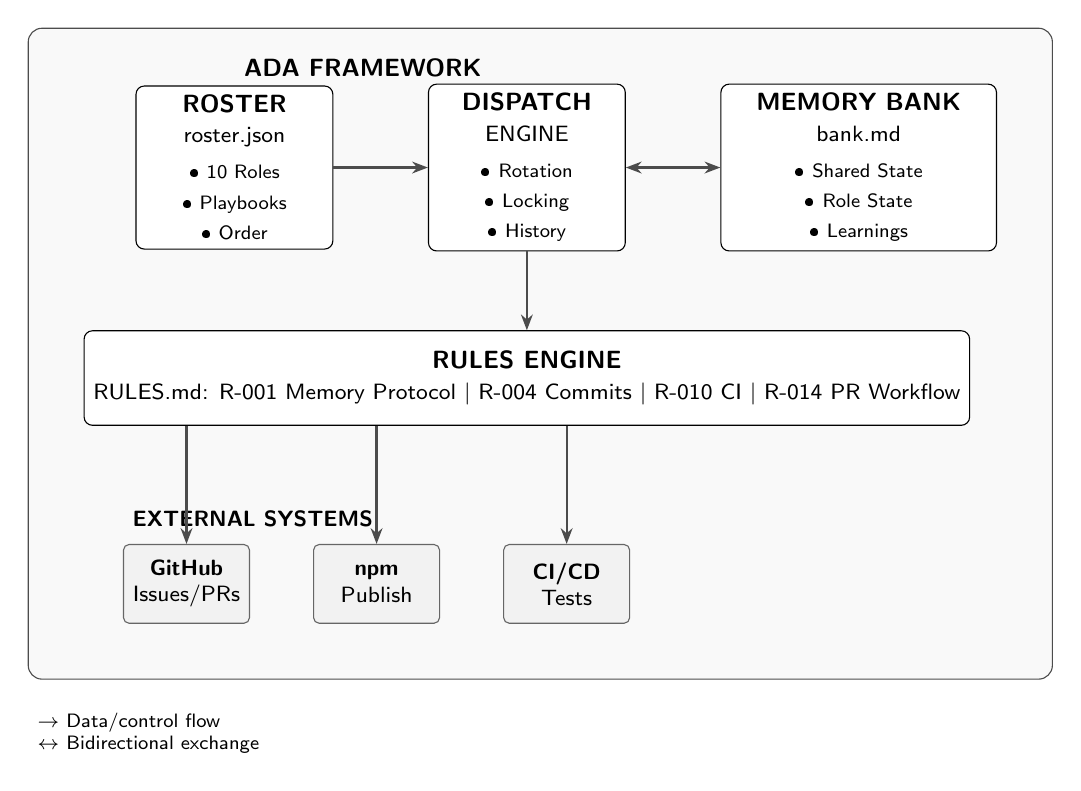
\begin{tikzpicture}[node distance=0.8cm]

% === CORE FRAMEWORK CONTAINER ===
\begin{scope}[local bounding box=framework]
    
    % Title
    \node[sectionlabel] at (0,0) {ADA FRAMEWORK};
    
    % Row 1: Roster, Dispatch, Memory
    \node[component] (roster) at (0,-1.5) {
        \textbf{ROSTER}\\
        \footnotesize roster.json\\[2pt]
        \scriptsize \textbullet~10 Roles\\
        \scriptsize \textbullet~Playbooks\\
        \scriptsize \textbullet~Order
    };
    
    \node[component, right=1.2cm of roster] (dispatch) {
        \textbf{DISPATCH}\\
        \footnotesize ENGINE\\[2pt]
        \scriptsize \textbullet~Rotation\\
        \scriptsize \textbullet~Locking\\
        \scriptsize \textbullet~History
    };
    
    \node[component, right=1.2cm of dispatch, minimum width=3.5cm] (memory) {
        \textbf{MEMORY BANK}\\
        \footnotesize bank.md\\[2pt]
        \scriptsize \textbullet~Shared State\\
        \scriptsize \textbullet~Role State\\
        \scriptsize \textbullet~Learnings
    };
    
    % Arrows between Row 1
    \draw[dataarrow] (roster.east) -- (dispatch.west);
    \draw[bidiarrow] (dispatch.east) -- (memory.west);
    
    % Row 2: Rules Engine (spanning)
    \node[component, below=1cm of dispatch, minimum width=9cm, minimum height=1.2cm] (rules) {
        \textbf{RULES ENGINE}\\
        \footnotesize RULES.md: R-001 Memory Protocol \textbar{} R-004 Commits \textbar{} R-010 CI \textbar{} R-014 PR Workflow
    };
    
    % Arrow from Dispatch to Rules
    \draw[dataarrow] (dispatch.south) -- (rules.north);
    
\end{scope}

% === EXTERNAL SYSTEMS CONTAINER ===
\node[external, below=1.5cm of rules.south west, anchor=north west, xshift=0.5cm] (github) {
    \textbf{GitHub}\\
    Issues/PRs
};

\node[external, right=0.8cm of github] (npm) {
    \textbf{npm}\\
    Publish
};

\node[external, right=0.8cm of npm] (ci) {
    \textbf{CI/CD}\\
    Tests
};

% External systems label
\node[sectionlabel, above=0.1cm of github.north west, anchor=south west] {\footnotesize EXTERNAL SYSTEMS};

% Arrows from Rules to External
\draw[dataarrow] (rules.south -| github.north) -- (github.north);
\draw[dataarrow] (rules.south -| npm.north) -- (npm.north);
\draw[dataarrow] (rules.south -| ci.north) -- (ci.north);

% === OUTER CONTAINER ===
\begin{pgfonlayer}{background}
    \node[container, fit=(roster)(dispatch)(memory)(rules)(github)(npm)(ci), inner sep=20pt] (outerbox) {};
\end{pgfonlayer}

% === LEGEND ===
\node[anchor=north west, font=\sffamily\scriptsize, text width=4cm] at ($(outerbox.south west)+(0,-0.3)$) {
    $\rightarrow$ Data/control flow\\
    $\leftrightarrow$ Bidirectional exchange
};

\end{tikzpicture}
\end{document}


\documentclass[tikz,border=10pt]{standalone}
\usepackage{tikz}
\usetikzlibrary{positioning,shapes.geometric,arrows.meta,fit,backgrounds,calc}

% Style definitions
\tikzset{
    % Main component boxes
    component/.style={
        draw=black,
        fill=white,
        rounded corners=3pt,
        minimum width=2.5cm,
        minimum height=1.8cm,
        align=center,
        font=\sffamily\small
    },
    % Large container boxes
    container/.style={
        draw=black!70,
        fill=gray!5,
        rounded corners=5pt,
        inner sep=12pt
    },
    % External system boxes
    external/.style={
        draw=black!60,
        fill=gray!10,
        rounded corners=2pt,
        minimum width=1.6cm,
        minimum height=1cm,
        align=center,
        font=\sffamily\footnotesize
    },
    % Section labels
    sectionlabel/.style={
        font=\sffamily\bfseries\small,
        anchor=north west
    },
    % Arrows
    dataarrow/.style={
        -{Stealth[length=2mm]},
        thick,
        black!70
    },
    bidiarrow/.style={
        {Stealth[length=2mm]}-{Stealth[length=2mm]},
        thick,
        black!70
    }
}

\begin{document}
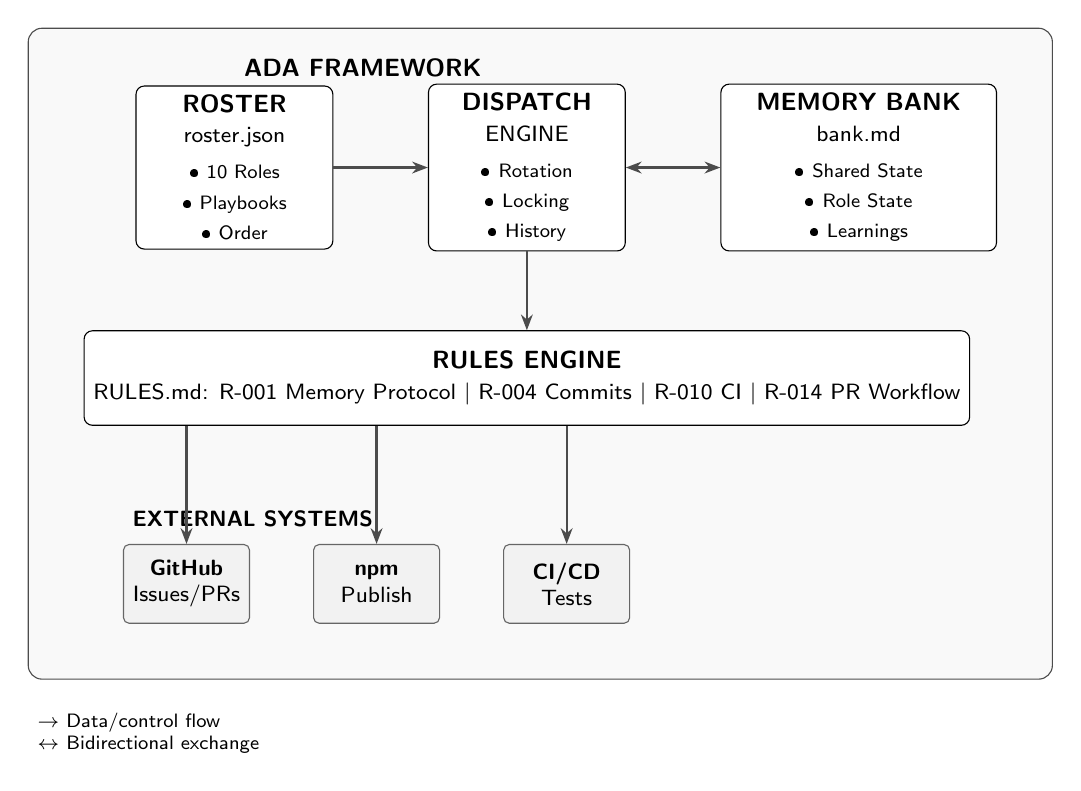
\begin{tikzpicture}[node distance=0.8cm]

% === CORE FRAMEWORK CONTAINER ===
\begin{scope}[local bounding box=framework]
    
    % Title
    \node[sectionlabel] at (0,0) {ADA FRAMEWORK};
    
    % Row 1: Roster, Dispatch, Memory
    \node[component] (roster) at (0,-1.5) {
        \textbf{ROSTER}\\
        \footnotesize roster.json\\[2pt]
        \scriptsize \textbullet~10 Roles\\
        \scriptsize \textbullet~Playbooks\\
        \scriptsize \textbullet~Order
    };
    
    \node[component, right=1.2cm of roster] (dispatch) {
        \textbf{DISPATCH}\\
        \footnotesize ENGINE\\[2pt]
        \scriptsize \textbullet~Rotation\\
        \scriptsize \textbullet~Locking\\
        \scriptsize \textbullet~History
    };
    
    \node[component, right=1.2cm of dispatch, minimum width=3.5cm] (memory) {
        \textbf{MEMORY BANK}\\
        \footnotesize bank.md\\[2pt]
        \scriptsize \textbullet~Shared State\\
        \scriptsize \textbullet~Role State\\
        \scriptsize \textbullet~Learnings
    };
    
    % Arrows between Row 1
    \draw[dataarrow] (roster.east) -- (dispatch.west);
    \draw[bidiarrow] (dispatch.east) -- (memory.west);
    
    % Row 2: Rules Engine (spanning)
    \node[component, below=1cm of dispatch, minimum width=9cm, minimum height=1.2cm] (rules) {
        \textbf{RULES ENGINE}\\
        \footnotesize RULES.md: R-001 Memory Protocol \textbar{} R-004 Commits \textbar{} R-010 CI \textbar{} R-014 PR Workflow
    };
    
    % Arrow from Dispatch to Rules
    \draw[dataarrow] (dispatch.south) -- (rules.north);
    
\end{scope}

% === EXTERNAL SYSTEMS CONTAINER ===
\node[external, below=1.5cm of rules.south west, anchor=north west, xshift=0.5cm] (github) {
    \textbf{GitHub}\\
    Issues/PRs
};

\node[external, right=0.8cm of github] (npm) {
    \textbf{npm}\\
    Publish
};

\node[external, right=0.8cm of npm] (ci) {
    \textbf{CI/CD}\\
    Tests
};

% External systems label
\node[sectionlabel, above=0.1cm of github.north west, anchor=south west] {\footnotesize EXTERNAL SYSTEMS};

% Arrows from Rules to External
\draw[dataarrow] (rules.south -| github.north) -- (github.north);
\draw[dataarrow] (rules.south -| npm.north) -- (npm.north);
\draw[dataarrow] (rules.south -| ci.north) -- (ci.north);

% === OUTER CONTAINER ===
\begin{pgfonlayer}{background}
    \node[container, fit=(roster)(dispatch)(memory)(rules)(github)(npm)(ci), inner sep=20pt] (outerbox) {};
\end{pgfonlayer}

% === LEGEND ===
\node[anchor=north west, font=\sffamily\scriptsize, text width=4cm] at ($(outerbox.south west)+(0,-0.3)$) {
    $\rightarrow$ Data/control flow\\
    $\leftrightarrow$ Bidirectional exchange
};

\end{tikzpicture}
\end{document}
